Table~\ref{tab:ga-tuning} shows that the settings change both mean cost and
run variation. All 330 runs returned feasible allocations. Every initial
population reached its target size, and none of the 101877 attempted offspring
repairs failed on these samples. These checks concern the generated workloads;
they do not establish a general feasibility guarantee for the decoder.
In the tuning runs, mean wall times were about 3.00 seconds at 100 tasks and 3.01 seconds at 200,
with a largest observed overrun of 0.093 seconds while an operation finished.

\begin{table}[htbp]
\centering
\small
\caption{GA settings at three seconds. Each size has three instances and five runs per setting. Cost and SD are in CU; SD is the average within instance sample standard deviation. Change is the mean paired percentage change from the default.}
\label{tab:ga-tuning}
\begin{tabular}{lrrrrrr}
\toprule
& \multicolumn{3}{c}{100 tasks, 12 servers} & \multicolumn{3}{c}{200 tasks, 24 servers} \\
\cmidrule(lr){2-4}\cmidrule(lr){5-7}
Setting & Cost & Change (\%) & SD & Cost & Change (\%) & SD \\
\midrule
Default & 1457.36 & $0.00$ & 14.63 & 2744.66 & $0.00$ & 14.13 \\
Population $N_{\rm pop}=12$ & 1444.89 & $-0.81$ & 29.31 & 2744.68 & $0.00$ & 30.49 \\
Population $N_{\rm pop}=48$ & 1457.63 & $+0.02$ & 14.15 & 2758.87 & $+0.53$ & 27.37 \\
Tournament $k=2$ & 1449.44 & $-0.51$ & 14.03 & 2751.49 & $+0.26$ & 12.89 \\
Tournament $k=5$ & 1446.25 & $-0.74$ & 25.74 & 2726.22 & $-0.67$ & 18.38 \\
Rank selection & 1447.78 & $-0.62$ & 27.87 & 2755.95 & $+0.41$ & 33.11 \\
Crossover $p_c=0$ & 1438.02 & $-1.27$ & 25.10 & 2731.35 & $-0.48$ & 22.12 \\
Crossover $p_c=0.6$ & 1442.30 & $-1.00$ & 23.91 & 2737.08 & $-0.29$ & 27.37 \\
Mutation $p_m=0$ & 1435.86 & $-1.44$ & 29.14 & 2732.71 & $-0.44$ & 18.96 \\
Mutation $p_m=0.01$ & 1435.62 & $-1.46$ & 29.94 & 2729.42 & $-0.55$ & 28.23 \\
Mutation $p_m=0.08$ & 1464.69 & $+0.52$ & 0.93 & 2775.86 & $+1.18$ & 23.15 \\
\bottomrule
\end{tabular}
\end{table}


\paragraph{Population and selection.}
Doubling the population from 24 to 48 did not improve mean cost at either size.
At 200 tasks its mean cost was 0.53\% higher than the paired default.
The smaller population of 12 improved the 100 task mean by 0.81\%, but made
almost no difference at 200 tasks and increased run variation. At 100 tasks,
populations 12, 24 and 48 completed means of 48.5, 20.4 and 9.8 full
generations; at 200 tasks the figures were 14.5, 6.3 and 2.8. A generation
contains a different number of children at each population size. The mean
accepted offspring counts were much closer: about 489, 458 and 473 at
100 tasks, and 150, 149 and 147 at 200. More generations therefore did not
mean a proportional increase in candidate allocations. Larger populations
also spent more of the allowance in initialisation.

Tournament size 5 lowered the paired mean by 0.74\% at 100 tasks and 0.67\%
at 200. Tournament size 2 and rank selection had lower means at 100 tasks
but slightly higher means at 200. Stronger selection was useful on these
tuning cases, although these differences are too limited to establish a
generally preferred selection rule.

\paragraph{Crossover and mutation.}
Skipping crossover improved the tuning means by 1.27\% and 0.48\%; using
crossover probability 0.6 improved them by 1.00\% and 0.29\%. These results
show that uniform crossover was not automatically helpful under this short
allowance and repair rule. They do not show that genetic recombination is
ineffective generally. The decoder still changes preferences and the local
pass still improves repaired children, even when crossover is skipped.

Mutation rate 0.01 had the lowest mean paired change when both sizes were
weighted equally: a 1.00\% reduction. Its mean costs were 1435.62 and
2729.42 CU, compared with the default's 1457.36 and 2744.66 CU.
The average within instance SD increased from 14.63 to 29.94 CU at
100 tasks and from 14.13 to 28.23 CU at 200. Thus a lower average cost
came with more variability. Mutation rate 0 was close behind on the tuning
criterion. The high rate 0.08 raised mean cost at both sizes. Its small
100 task SD of 0.93 CU describes consistency, but that consistency came
with a more expensive mean allocation.

Figure~\ref{fig:ga-settings} retains the differences between workloads.
For mutation rate 0.01, the paired improvements at 100 tasks were 0.16\%,
1.25\% and 2.97\% on seeds 11, 22 and 33. The latter two cases saved mean
activation charges of 20.2 and 48.0 CU, while paying slightly more in
assignment charges. Occasional better consolidation therefore accounts for
much of the mean improvement. The effect is not uniform across instances.

One possible explanation is that independent crossover and resets disrupt
groups of tasks sharing a cheap server. A feasible repair need not restore
those groups, and a single task move cannot always empty a server whose
tasks would have to move together. This interpretation agrees with the
observed cost components: at 200 tasks, mutation rate 0.08 paid a mean
31.2 CU more in activation charges than the default, while their mean
assignment charges were almost identical. The experiment does not isolate
each mechanism, so it supports this explanation without proving it.

\begin{figure}[htbp]
\centering
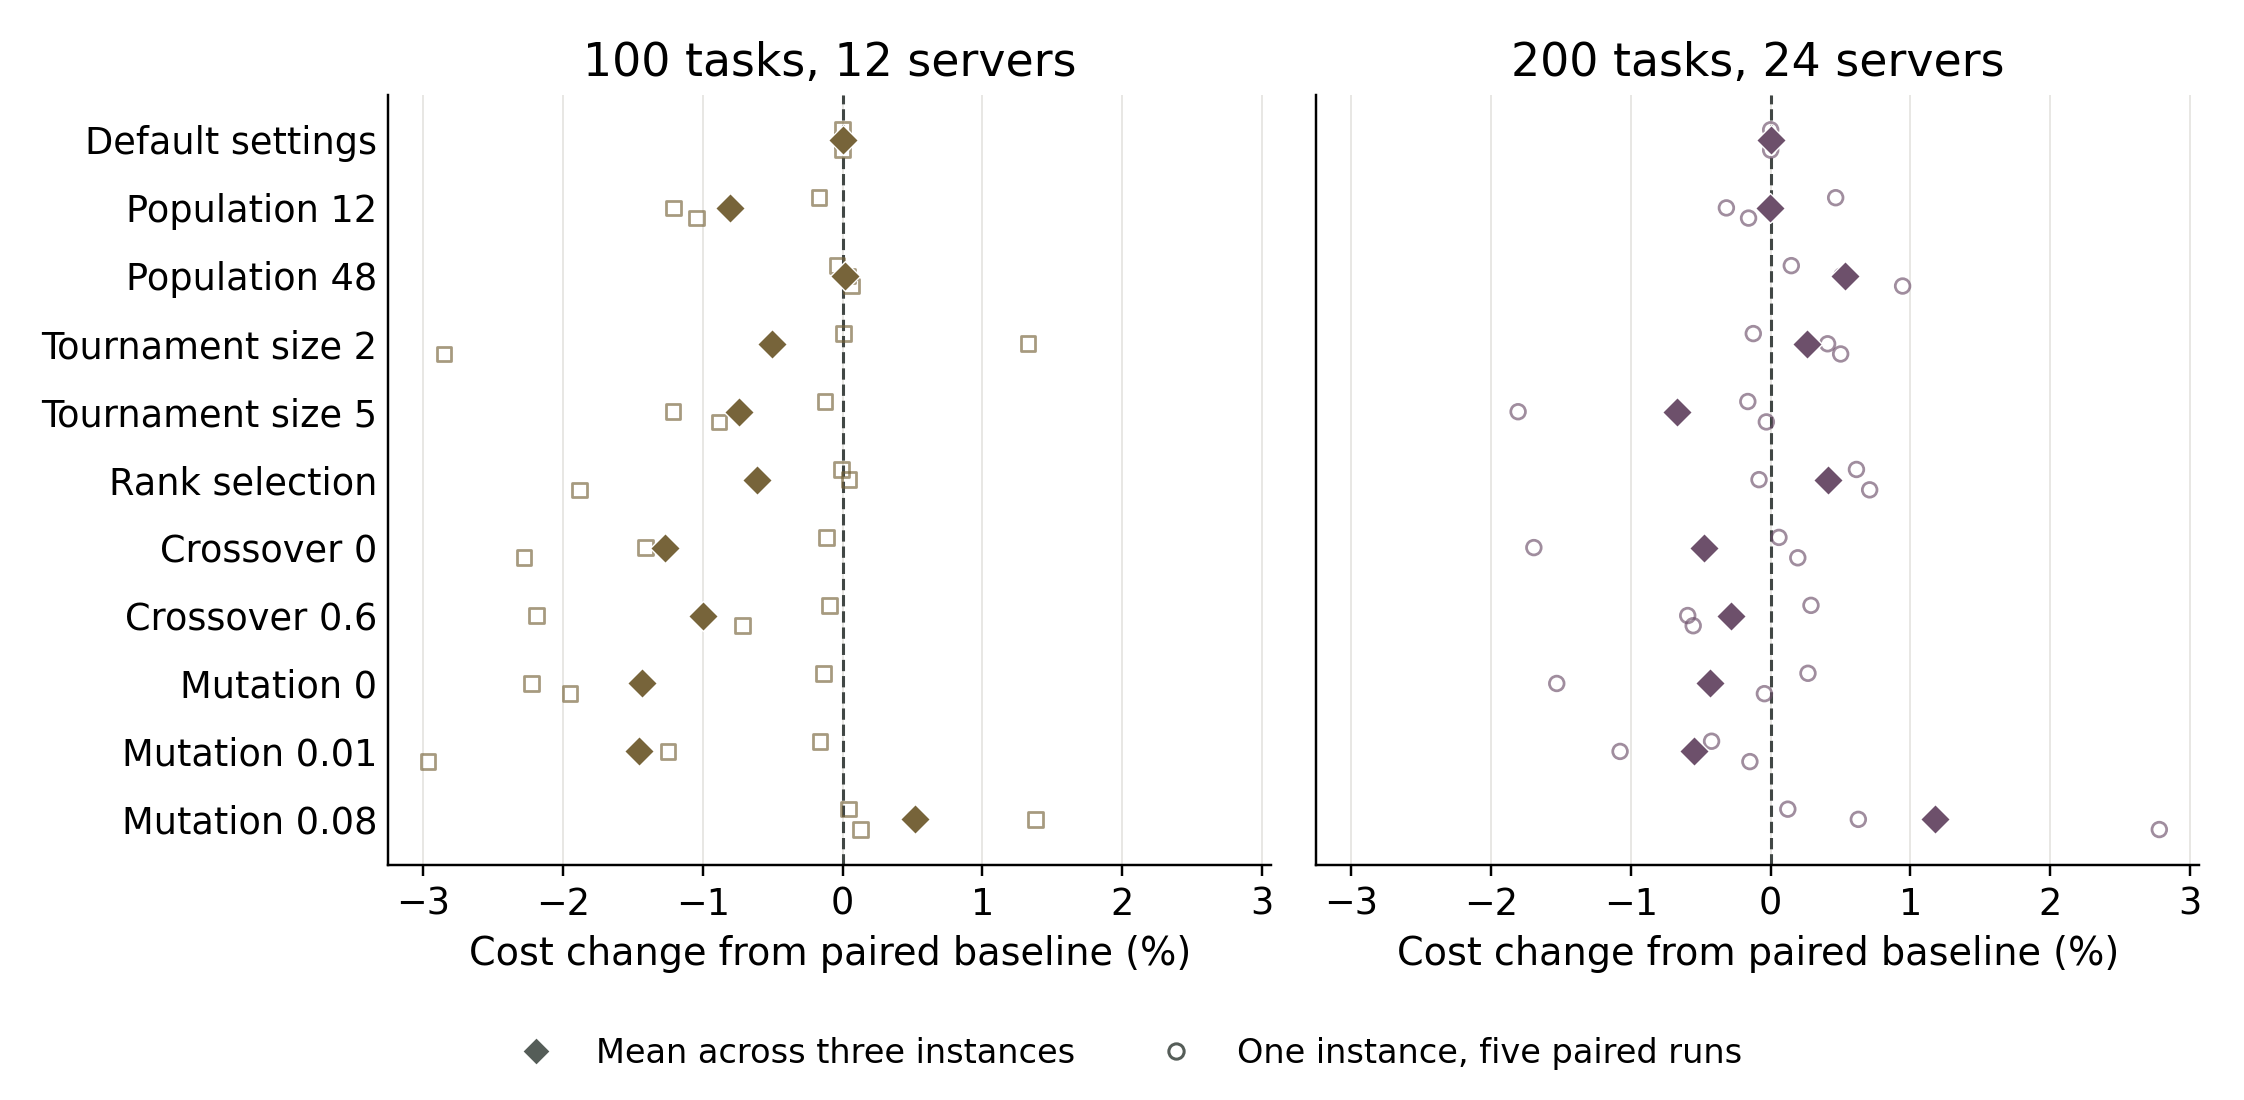
\includegraphics[width=\textwidth]{ga_tuning/parameter_changes.png}
\caption{Paired changes in GA cost at three seconds. Each hollow marker is an
instance's mean across five paired runs; each solid diamond averages the three
instance means. Negative values favour the changed setting. These markers
describe instance variation, not confidence intervals.}
\label{fig:ga-settings}
\end{figure}

\paragraph{Validation on new instances.}
The selected setting changes only $p_m$ to 0.01. Table~\ref{tab:ga-validation}
uses seeds 44, 55 and 66, which were excluded from selection. All 60
validation runs were feasible. The pooled paired change was $+0.006\%$,
effectively zero: $+0.020\%$ at 100 tasks and $-0.007\%$ at 200 tasks.
The selected setting had a lower mean cost on three of the six workloads
and won 17 of the 30 paired runs. These repeated runs share only six
workloads, so they are not 30 independent tests of transfer to different data.

\begin{table}[htbp]
\centering
\small
\caption{Validation on unseen instance seeds at three seconds, with five runs per cell. SD is the sample standard deviation within that instance, in CU. Changes pair identical instance and run seeds.}
\label{tab:ga-validation}
\begin{tabular}{rrrrrrr}
\toprule
Tasks & Seed & Default (CU) & Selected (CU) & Change (\%) & Default SD & Selected SD \\
\midrule
100 & 44 & 1582.65 & 1583.13 & $+0.03$ & 1.64 & 1.42 \\
100 & 55 & 1320.61 & 1318.80 & $-0.14$ & 2.31 & 3.72 \\
100 & 66 & 1532.72 & 1535.25 & $+0.17$ & 2.47 & 1.97 \\
200 & 44 & 2800.63 & 2800.11 & $-0.02$ & 4.42 & 1.15 \\
200 & 55 & 2787.57 & 2793.37 & $+0.21$ & 18.19 & 19.57 \\
200 & 66 & 2881.72 & 2875.44 & $-0.22$ & 3.53 & 11.14 \\
\bottomrule
\end{tabular}
\end{table}


The tuning gain did not transfer consistently to the new seeds. I therefore
retain the original default rate for the main comparison and treat 0.01 as
a candidate for a particular workload, rather than a generally improved
setting. The validation set was not used to choose a second winner.
This outcome is useful: settings that look favourable on a small tuning set
can make almost no difference on another set from the same generator.
The study is limited to three seconds, two sizes and one parameter at a time;
it does not identify an optimum over all GA settings or their interactions.

\Needspace{7\baselineskip}
The validation can be repeated with the study script using
\begin{verbatim}
python3 run_ga_study.py --phase validation \
  --configs baseline mutation_001 --budget 3 \
  --repetitions 5 --output ga_validation_new
\end{verbatim}
The raw records, saved assignments and improvement traces support these
comparisons, including the validation result that did not favour the tuning
winner overall.
